%
% Document class
\documentclass[9pt]{beamer}
%
% Theme
\usetheme[
numbering=fraction,
% background=dark,
progressbar=foot,
]{metropolis}
%
% Colors
\definecolor{murraygold}{RGB}{240,195,58}
\definecolor{murrayblue}{RGB}{2,8,69}
\setbeamercolor{normal text}{bg=white,fg=murrayblue}
\setbeamercolor{alerted text}{fg=murraygold}
\setbeamercolor{example text}{fg=murraygold}
%
% Detailed settings/packages
%
% General packages
\usepackage{textpos}
% \usepackage{fontspec}
%
% Location(s) of images
\graphicspath{{images/}}
%
% Fonts
\setsansfont[BoldFont={Fira Sans SemiBold}]{Fira Sans}
\setbeamerfont{title}{size=\huge}
\setbeamerfont{author}{size=\LARGE}
\setbeamerfont{date}{size=\normalsize}
\setbeamerfont{institute}{size=\normalsize}
\setbeamerfont{frametitle}{series=\mdseries}
%
% Margins
% \setbeamersize{text margin left=0.5cm,text margin right=0.5cm}
%
% Frame title logo
\makeatletter
\newlength{\frametitleheight}% <- NEW
\newsavebox{\beamer@titlebox}% <- NEW
\setbeamertemplate{frametitle}{%
  \ifbeamercolorempty[bg]{frametitle}{}{\nointerlineskip}%
  \@tempdima=\textwidth%
  \advance\@tempdima by\beamer@leftmargin%
  \advance\@tempdima by\beamer@rightmargin%
  \sbox{\beamer@titlebox}{% <- NEW
      \begin{beamercolorbox}[sep=0.3cm,left,wd=\the\@tempdima]{frametitle}
        \usebeamerfont{frametitle}%
        \vbox{}\vskip-1ex%
        \if@tempswa\else\csname beamer@fteleft\endcsname\fi%
        \strut\insertframetitle\strut\par%
        {%
          \ifx\insertframesubtitle\@empty%
          \else%
          {\usebeamerfont{framesubtitle}\usebeamercolor[fg]{framesubtitle}\insertframesubtitle\strut\par}%
          \fi
        }%
        \vskip-1ex%
        \if@tempswa\else\vskip-.3cm\fi% set inside beamercolorbox... evil here...
      \end{beamercolorbox}%
     }% <- NEW
     \usebox{\beamer@titlebox}% <- NEW
\settoheight{\frametitleheight}{\usebox{\beamer@titlebox}}% <- NEW
\addtolength{\frametitleheight}{\headheight}}
\makeatother
\addtobeamertemplate{frametitle}{}{%
  \begin{tikzpicture}[remember picture,overlay]
    \node[inner sep=0, outer sep=0, anchor= east,xshift=-2mm,yshift=-0.5*\frametitleheight] at (current page.north east) {\includegraphics[height=0.675cm, keepaspectratio]{murraystate-logo-shield.png}};
  \end{tikzpicture}}
%
% Progress bar width
\makeatletter
\setlength{\metropolis@progressinheadfoot@linewidth}{1pt}
\makeatother
%
% Footer
\setbeamertemplate{frame footer}{\vspace*{-5pt}\insertshorttitle\hfill\secname}
\setbeamerfont{page number in head/foot}{size=\tiny}
\setbeamercolor{footline}{fg=gray}
%
%%% Local Variables:
%%% mode: latex
%%% TeX-master: "git-tutorial"
%%% TeX-engine: xetex
%%% End:

%
% Document information
\title{Version Control}
\date{\today}
\author{Tyler D. Stoffel}
\institute{ENT 419: Senior Project I}
\titlegraphic{\vspace*{7.25cm}\includegraphics[width=4cm]{murraystate-logo-primary.png}}
%
% Start document
\begin{document}
\maketitle
%
% \section{First Section}
%
\begin{frame}{Version control}
  \begin{columns}
    \begin{column}{0.6\linewidth}
      What is version control?
      \begin{itemize}
        \item The traditional way: New version? \\ \emph{File $\rightarrow$ Save as $\rightarrow$ myDocument\_v2.docx}
        \item The better way: Version control.
      \end{itemize}
      \begin{alertblock}{Version control}
       A system that records changes to files over time so that you can recall specific versions, merge changes, collaborate on developing the files, and more.
      \end{alertblock}
      Some programs that have version control built in:
      \begin{itemize}
        \item AutoCAD and SolidWorks
        \item
      \end{itemize}
    \end{column}
    \begin{column}{0.4\linewidth}
      \begin{figure}
        \centering
        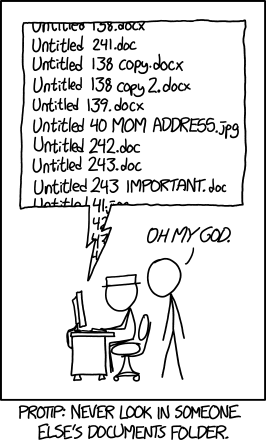
\includegraphics[width=3.5cm]{version-control-comic.png}
        \caption{The traditional way.}
      \end{figure}
    \end{column}
  \end{columns}
\end{frame}
%
\begin{frame}{What is \texttt{git}?}
  \begin{itemize}
    \item Created by Linux Torvalds, creator of Linux, in 2005.
  \end{itemize}
\end{frame}
%
\end{document}
%
%%% Local Variables:
%%% mode: latex
%%% TeX-master: t
%%% End:
